\documentclass{article}
\usepackage[preprint]{tmlr}
\usepackage{amsmath,amssymb,booktabs,tabularx,array,graphicx}
\usepackage{hyperref}
\usepackage{url}
% Permit breaks inside pinned hexadecimal hashes without changing their URLs.
\makeatletter
\g@addto@macro\UrlBreaks{\do\a\do\b\do\c\do\d\do\e\do\f\do\0\do\1\do\2\do\3\do\4\do\5\do\6\do\7\do\8\do\9}
\makeatother
\Urlmuskip=0mu plus 1mu\relax
\hypersetup{colorlinks=true,citecolor=blue,linkcolor=blue,urlcolor=blue}

\title{TR-HASH: Composed Modulo Routing for\\Sequential Adaptation}
\author{Boris Peyriguere\\Local working manuscript}
\date{}

\newcommand{\RMS}{\operatorname{RMSNorm}}
\newcommand{\RoPE}{\operatorname{RoPE}}
\newcommand{\softmax}{\operatorname{softmax}}
\newcommand{\silu}{\operatorname{SiLU}}
\newcommand{\Ind}{\mathbf{1}}
\newcommand{\Source}{\textsc{TR-HASH}}
\newcommand{\TR}{\textsc{TR-HASH}}
\newcommand{\CE}{\mathcal{L}}

\begin{document}
\maketitle

\begin{abstract}
We document a small deterministic-routing language model and the limits of its saved development evidence. The frozen \Source{} configuration has two layers, hidden width $64$, four query heads sharing one key/value head, and $110{,}976$ trainable parameters. Each feedforward block combines a shared SwiGLU with two of four experts. Expert identities depend on the current byte and two previous byte identities; separate current-byte rules select attention outputs, and a cyclic input permutation affects only the first value projection. Under a fixed language-modeling, continuation, and supervised-adaptation protocol, the selected archived candidate satisfies a $0.001$-nat margin in $67$ of $70$ comparisons against two original dense references and $30$ of $35$ against a dense control with the same attention/value transformations. The combined $97/105$ score fails the all-comparisons objective; reserved confirmation remains closed. These are exploratory observations after repeated selection on seven development seeds, not independent evidence of general superiority. A completed $28$-trajectory development qualification adds a learned shared-plus-routed MoE with $111{,}488$ parameters, a $0.461\%$ increase. The deterministic model has the lowest mean on all five metrics and meets $98/105$ margin comparisons against three freshly trained controls, with five clear losses and two near-equal cases. These new comparisons reuse the development seeds and splits; they do not supply independent confirmation. We provide an executable architectural specification and a provenance-linked account of both favorable averages and failed comparisons.
\end{abstract}

\section{Introduction}
Conditional feedforward computation can separate stored model capacity from the subset of experts assigned to an input. Learned gating is a prominent way to make this assignment \citep{shazeer2017moe,fedus2022switch}. Here we examine a different choice: routes computed entirely from byte identities and a short causal history. The shared branch remains active for every position, and every parameter remains trainable. The question is whether this particular organization helps preserve language-modeling performance through a subsequent instruction-adaptation stage at a small, closely controlled parameter budget.

The scope is deliberately narrow. The empirical system is a $110{,}976$-parameter byte-level decoder trained on a small Shakespeare language-modeling split and $512$ filtered Alpaca instruction examples. This is a sequential adaptation experiment, not a competitive general-purpose language-model benchmark. Response cross-entropy is measured, but no human preference score, reasoning benchmark, or generation-quality ranking is available. ``Retention'' denotes a specified difference between two held-out language-modeling losses; it does not establish that particular facts, skills, or representations have been protected.

This manuscript distinguishes two evidence sets. The \emph{observed archive} contains a selected \Source{} candidate, historical original dense references, and its contemporaneous matched dense control. The completed \emph{four-model qualification} trains four architectures afresh, including a learned MoE inspired by the shared/routed decomposition described in Qwen2 \citep{yang2024qwen2}. The latter is a small local control, not an official Qwen model or a reproduction of its training. Its $98/105$ grid uses controls $E,D,$ and learned MoE, whereas the archive's $97/105$ grid uses $E,C,D$. These are different denominators and must remain distinct.

The archived candidate meets $97$ of $105$ binary development comparisons, while the declared objective requires all $105$. The failures are substantive: three original-reference comparisons fail on forgetting, and five additional failures remain against the matched control. Moreover, promoting the candidate from the preceding reference improves the selected win count while worsening mean response loss. These facts motivate reporting the exact recipe and its counterexamples together, rather than treating a large aggregate win count as a universal result.

Our contributions are therefore limited to (i) an unambiguous specification of the two-layer routing and attention transformations; (ii) a provenance-linked description of saved development metrics, including the failed objective and selection limitations; and (iii) a completed, near-parameter-matched learned-router comparison with a fixed data and optimization contract. Document preparation itself performs no training or model evaluation.

\section{Frozen architecture}
\label{sec:architecture}
\subsection{Backbone and notation}
Let $t_i\in\{0,\ldots,255\}$ be the original UTF-8 byte identity at position $i$. Token identities are preserved for routing even after the hidden representation has been contextualized. The experimental decoder has hidden width $H=64$, depth $L=2$, maximum context $256$, four query heads, and one key/value head, with head dimension $d=16$. This is the single-KV, or multi-query, endpoint of the grouped-query attention interface \citep{ainslie2023gqa}. It is useful to state the counts explicitly rather than implying that several KV groups are used.

A tied byte embedding provides both input vectors and output logits. There are no linear-layer biases. Each block uses pre-normalized residual attention followed by a pre-normalized residual feedforward transformation. Hidden-state and per-head normalizers are RMSNorm \citep{zhang2019rmsnorm}, with $\epsilon=10^{-6}$:
\begin{equation}
 \RMS(z)=\gamma\odot z\left(\frac{1}{D}\sum_{j=1}^{D}z_j^2+10^{-6}\right)^{-1/2}.
\end{equation}
A final hidden-state RMSNorm precedes the tied output projection. Dropout is zero. The numerical reference uses full causal attention rather than a sliding window.

\subsection{Shared and routed SwiGLU}
For intermediate width $w$, write a bias-free SwiGLU \citep{shazeer2020glu} as
\begin{equation}
 F_w(x)=W_{\mathrm{down}}\bigl(\silu(W_{\mathrm{gate}}x)\odot W_{\mathrm{up}}x\bigr).
\end{equation}
At layer $\ell$, the shared function $S_\ell$ has width $128$. Four independent expert functions $E_{\ell,e}$ have width $16$ each. Given two distinct expert identities $a_{\ell,i},b_{\ell,i}$, the feedforward output is
\begin{equation}
 M_\ell(x_i,t_{\le i})=S_\ell(x_i)+2\left[\tfrac12 E_{\ell,a_{\ell,i}}(x_i)+\tfrac12 E_{\ell,b_{\ell,i}}(x_i)\right].
 \label{eq:mlp}
\end{equation}
Thus the fixed branch scales are $1$ for the shared output and $2$ for the routed mixture. The $50/50$ mixture and multiplier $2$ must be considered together: each selected expert has effective coefficient $1$. This is not an average of the shared branch and the two experts. The reference has no learned routing logits, learned branch gate, or load-balancing term.

\subsection{Two-lag expert identities}
Set missing preceding identities to zero at the start of each input sequence, and define
\begin{equation}
 u_i=(t_{i-1}+5t_{i-2})\bmod9.
 \label{eq:history}
\end{equation}
The two MLP layers have different rules. For layer $0$,
\begin{align}
 a_{0,i}&=t_i\bmod4,\\
 s_{0,i}&=1+\left(\left\lfloor t_i/4\right\rfloor+(u_i\bmod3)\right)\bmod3,\\
 b_{0,i}&=(a_{0,i}+s_{0,i})\bmod4.
 \label{eq:m0}
\end{align}
For layer $1$,
\begin{align}
 a_{1,i}&=((t_i+1)\bmod4)\mathbin{\oplus_{\rm bit}}\left[2\bigl((u_i\bmod3)\bmod2\bigr)\right],\\
 s_{1,i}&=1+\left(\left\lfloor t_i/4\right\rfloor+2\left\lfloor u_i/3\right\rfloor+1\right)\bmod3,\\
 b_{1,i}&=(a_{1,i}+s_{1,i})\bmod4.
 \label{eq:m1}
\end{align}
Here $\oplus_{\rm bit}$ denotes bitwise XOR. The quantities entering it lie in $\{0,1,2,3\}$ and $\{0,2\}$. In both layers, $s\in\{1,2,3\}$ guarantees distinct experts. The layer $1$ rule changes both primary selection and the secondary offset as a function of the short identity history. The routing functions are causal, but they are not learned functions of hidden activations. ``Hash'' is a historical system name for these composed-modulo assignments, not a cryptographic property.

\subsection{Value-input binding and attention-head selection}
For an RMS-normalized attention input $x_i\in\mathbb{R}^{64}$, define a byte-dependent cyclic coordinate read
\begin{equation}
 (P_{t_i}x_i)_j=(x_i)_{(j+16(t_i\bmod4))\bmod64},\qquad j=0,\ldots,63.
 \label{eq:v0}
\end{equation}
Only the layer $0$ value projection receives $P_{t_i}x_i$. Layer $1$ values receive $x_i$ unchanged, and query/key inputs are unchanged in both layers. Each $P_t$ is a permutation, preserving the input norm, but its composition with a learned value projection can still change attention behavior. This arithmetic operation is not a claim about semantic token classes.

Query and key projections receive last-dimension RMSNorm before rotary positional transformation \citep{su2021roformer}. The query normalizer has one learned $16$-vector shared across query heads; the key normalizer has a separate $16$-vector. Rotary positions use base $10{,}000$ with the source split-half layout. With the one shared key/value head,
\begin{equation}
 q_{i,h}=\RoPE_i(\RMS_Q(W_{Q,h}x_i)),\quad
 k_i=\RoPE_i(\RMS_K(W_Kx_i)),\quad
 v_i=W_VP^{(\ell)}_{t_i}x_i,
\end{equation}
where $P^{(0)}_t=P_t$ and $P^{(1)}_t=I$. Every query head first computes the usual causal output $y_{i,h}=\sum_{j\le i}\softmax_j(q_{i,h}^{\mathsf T}k_j/\sqrt{16})v_j$.

The selected head identities are separate from the MLP routes. Layer $0$ uses
\begin{equation}
 c_{0,i}=t_i\bmod4,\qquad
 d_{0,i}=\left(c_{0,i}+1+\lfloor t_i/4\rfloor\bmod3\right)\bmod4.
\end{equation}
Layer $1$ instead uses the current-ID-only adjacent pair
\begin{equation}
 c_{1,i}=\left\lfloor t_i/12\right\rfloor\bmod4,\qquad
 d_{1,i}=(c_{1,i}+1)\bmod4.
 \label{eq:head1}
\end{equation}
After attention, before the shared output projection, the retained outputs are
\begin{equation}
 \widetilde y_{i,h}=\sqrt{2}\,
 \Ind\{h\in\{c_{\ell,i},d_{\ell,i}\}\}\,y_{i,h},\qquad
 A_\ell(x)_i=W_O\operatorname{concat}_{h=0}^{3}\widetilde y_{i,h}.
 \label{eq:headmask}
\end{equation}
The $\sqrt2$ factor is part of the fixed recipe. It does not imply exact variance preservation for correlated, learned heads. Neither head rule uses the two-lag context in Equation~\ref{eq:history}; that context belongs to the MLP. This distinction is necessary to reproduce the candidate.

\subsection{Capacity and computational scope}
The shared and expert FFNs store the same number of parameters as one width-$192$ dense SwiGLU: $3H(128+4\cdot16)=3H\cdot192$. With tied embeddings, two attention blocks, and normalizers, each original comparison architecture stores $110{,}976$ trainable parameters. The reference evaluates all expert functions before applying assignment weights, and computes all query-head outputs before applying Equation~\ref{eq:headmask}. It therefore demonstrates neither sparse-kernel acceleration nor a reduction in realized FLOPs. Assignment sparsity, stored capacity, theoretical active capacity, and measured execution cost are distinct quantities in this study.

\section{Data, optimization, and recorded comparisons}
\label{sec:protocol}
\subsection{Fixed small-data protocol}
Table~\ref{tab:protocol} records the complete stage schedule. All experiments operate on UTF-8 bytes, not a learned subword vocabulary. The language-modeling source is the pinned Tiny Shakespeare file distributed with \texttt{char-rnn}; its first $90\%$ of bytes and final $10\%$ define the source training/validation regions \citep{karpathy2015charrnn}. Within each region, the frozen loader forms $129$-byte windows at stride $128$, permutes their indices with data seed $42$, and selects $2{,}048$ training and $256$ validation windows. Each window supplies $128$ next-byte targets. No byte window crosses the source-region boundary.

The instruction source is a pinned Stanford Alpaca JSON file \citep{taori2023alpaca}. The loader keeps examples with empty auxiliary input, nonempty instruction/answer strings, and a complete encoded sequence of at most $256$ bytes. It removes duplicate instructions using normalized case and whitespace, shuffles the eligible set with data seed $42$, and takes $512$ training examples followed by $128$ validation examples. The exact prompt is \texttt{Instruction: \{instruction\}\textbackslash nAnswer: } followed by the answer and a newline. Prompt positions and batch-padding positions are excluded from the response loss. These filtering choices are part of this local protocol, not an evaluation of the full Alpaca collection.

\begin{table}[t]
\centering
\caption{Frozen training schedule per trajectory. Refinement is a continuation on the same fixed language-modeling training set. During SFT there is no language-modeling replay. Each stage starts a new AdamW optimizer. Counts denote supervised next-byte targets, including repeated epochs.}
\label{tab:protocol}
\begin{tabular}{lrrrr}
\toprule
Stage & Epochs & Learning rate & Updates & Target presentations\\
\midrule
Language pretraining & 2 & $10^{-3}$ & 256 & $524{,}288$\\
LM refinement & 1 & $5\cdot10^{-4}$ & 128 & $262{,}144$\\
Instruction SFT & 12 & $2\cdot10^{-4}$ & 384 & $452{,}292$\\
\midrule
Total & & & 768 & $1{,}238{,}724$\\
\bottomrule
\end{tabular}
\end{table}

Batch size is $16$. The fixed LM and SFT training lists contain $128$ and $32$ batches respectively; the order is retained rather than reshuffled every epoch. There are $262{,}144$ supervised LM targets and $37{,}691$ supervised SFT targets before epoch repetition. Their validation counterparts contain $32{,}768$ and $9{,}386$ targets. All trainable weights continue to update in all stages. Stable routing is not a parameter-freezing mechanism.

AdamW \citep{loshchilov2019adamw} uses $\beta=(0.9,0.999)$, $\epsilon=10^{-8}$ and weight decay $0.01$, with no gradient clipping in the frozen training functions. Stage transitions reset optimizer state. The source initialization uses normal weights with standard deviation $0.02$, reduced by $\sqrt{2L}=2$ for residual output projections, and standard unit RMSNorm scales. The frozen reference environment is CPU float32, four Torch threads, deterministic algorithms enabled, highest float32 matmul precision, and Torch $2.13.0$. The model seeds are
\begin{equation}
 \mathcal S=(42,123,314,159,265,358,979),
\end{equation}
while data seed $42$ stays fixed. Repeating these seeds changes initialization, not the selected examples or data ordering.

\subsection{Metrics and the declared gate}
At the end of each stage, the frozen procedure evaluates language-modeling and response-validation cross-entropy, normalized by their supervised next-byte targets. The five reported endpoint metrics are $\CE_{\mathrm{pre}}$, $\CE_{\mathrm{ref}}$, $\CE_{\mathrm{LM,SFT}}$, $\CE_{\mathrm{response,SFT}}$, and
\begin{equation}
 F=\CE_{\mathrm{LM,SFT}}-\CE_{\mathrm{ref}}.
 \label{eq:forgetting}
\end{equation}
Lower values are preferred for all five quantities. A lower forgetting difference by itself could reflect a worse pre-adaptation reference loss; it must therefore be read together with both endpoint losses. These are conditional cross-entropies in nats per target byte, not accuracy scores.

For seed $s$, metric $m$, and comparator $a$, the archived win convention is
\begin{equation}
 w_{s,m,a}=\Ind\{\CE_{s,m,\TR}-\CE_{s,m,a}\le -0.001\}.
 \label{eq:win}
\end{equation}
Here $\CE$ also denotes the forgetting metric when $m=F$. The original-reference count has $7\cdot5\cdot2=70$ comparisons; a separate matched-control count has $7\cdot5=35$. The declared gate requires all $105$ comparisons to satisfy Equation~\ref{eq:win}. This gate is a development convention, not a statistical significance test. Metrics share models and datasets, and forgetting is algebraically dependent on two losses, so the $105$ comparisons are not $105$ independent observations.

\subsection{Identity of the archived controls}
The observed candidate, denoted $B_{63}$, and matched control $D_{63}$ were each trained fresh on the seven seeds in the completed Source63 run. $D_{63}$ replaces the expert MLP with width-$192$ dense SwiGLU while retaining the candidate's routed attention outputs, first-layer value-input permutation, and unchanged backbone dimensions. Its comparison is the closest available control for the MLP organization at that attention setting.

The original controls are $E$, a width-$192$ dense FFN with all attention heads retained and no value-input permutation, and $C$, a dense FFN with the earlier composed head rule and no value-input permutation. Their saved trajectories originate from earlier development lots and were reused as frozen references; they were not retrained in lot $63$. All four archived architectures have $110{,}976$ parameters, but their attention/value transformations differ. Consequently, the original $70$ comparisons do not isolate expert routing alone.

\section{Saved development observations}
\label{sec:observations}
\subsection{Endpoint losses and margin counts}
The archive's candidate $B_{63}$ has lower means on all five metrics than $E$, $C$, and $D_{63}$. Fresh $T,E,D$ means in Table~\ref{tab:freshmeans} exactly reproduce their historical counterparts. The historical $C$ means are $2.24387$ (LM pretraining), $2.12465$ (refinement), $2.44837$ (LM after SFT), $2.35662$ (response), and $0.32372$ (forgetting). No model was evaluated during manuscript preparation. The per-seed gate nevertheless fails, as Table~\ref{tab:wins} makes explicit.

\begin{table}[t]
\centering
\caption{Saved wins under the fixed $0.001$-nat convention. The original references contribute $14$ seed--comparator entries per metric and the matched control contributes $7$. Both gates remain false.}
\label{tab:wins}
\begin{tabular}{lrr}
\toprule
Metric & Against $E,C$ & Against $D_{63}$\\
\midrule
LM pretraining & $14/14$ & $7/7$\\
LM refinement & $14/14$ & $7/7$\\
LM after SFT & $14/14$ & $6/7$\\
Response after SFT & $14/14$ & $6/7$\\
Forgetting & $11/14$ & $4/7$\\
\midrule
Total & $67/70$ & $30/35$\\
All-comparisons gate & false & false\\
\bottomrule
\end{tabular}
\end{table}

The counts against $E$ and $C$ are $34/35$ and $33/35$ respectively. All three failures in the original-reference count concern forgetting: seed $265$ against $E$, and seeds $314$ and $159$ against $C$. Their candidate-minus-control differences are $+0.019619$, $+0.013082$, and $+0.033240$ nats. These are losses relative to the comparator, not cases just missing an otherwise favorable margin.

The matched-control failures include forgetting at seeds $314$, $265$, and $358$, LM-after-SFT loss at seed $314$, and response loss at seed $42$. The latter has difference $+0.000929$; it fails both the required negative margin and simple lower-loss ordering. The combined score is $97/105$, leaving eight failed comparisons. The archive marks the global objective false and confirmation calls zero. Averaging losses cannot turn this into an all-seeds, all-metrics success.

\subsection{Selection and the preceding reference}
Source63 was promoted because the original-reference count rose from $66/70$ for the preceding Source42 reference to $67/70$, with its fixed original win set retained. The additional win is forgetting against $E$ at seed $979$. The matched-control count remains $30/35$. This is a precise description of the promotion rule, not an independently tested discovery criterion.

The promotion is not a Pareto improvement over Source42. The archived descriptive comparison reports four lower mean metrics but a $+0.00385052$ increase in mean response loss, with four of seven seeds worse on that metric. The changed layer $1$ head law also changes primary-head selection and adjacency jointly relative to the previous rule. The archive does not isolate an effect of the quotient, adjacency, expert routing, or value permutation individually. Those mechanisms require separate matched interventions.

A historical $17/20$ result is preserved from a two-seed, earlier $50/50$ context-routing protocol. It is not a subset to add to $97/105$, a replication of Source63, or an independent confirmation. Its protocol, checkpoints, and source strings are retained solely as lineage evidence.

\section{Completed four-model development qualification}
\label{sec:qualification}
\subsection{Architecture matrix and budget}
The completed qualification contains $28$ fresh trajectories: four architectures on all seven listed seeds, each initialized before its full pretraining--refinement--SFT sequence. Table~\ref{tab:qualification} states the executed matrix. The former original-head control $C$ is not one of these four fresh architectures. Its historical scores must not be silently transferred to another model.

\begin{table}[t]
\centering
\caption{Completed qualification architectures, seven seeds each. All use $H=64$, $L=2$, four query heads and one KV head. ``Fixed attention/V0'' means the candidate's head mask and value-input permutation. The learned control adds $512$ router parameters.}
\label{tab:qualification}
\begin{tabularx}{\textwidth}{@{}lXcr@{}}
\toprule
Model & Feedforward organization & Fixed attention/V0 & Parameters\\
\midrule
$T$ & shared $128$ + four experts $16$; identity-history top-$2$ & yes & $110{,}976$\\
$E$ & dense SwiGLU $192$ & no & $110{,}976$\\
$D$ & dense SwiGLU $192$ & yes & $110{,}976$\\
$M$ & shared $128$ + four experts $16$; learned top-$2$ & yes & $111{,}488$\\
\bottomrule
\end{tabularx}
\end{table}

The learned control borrows the general shared-plus-routed expert organization discussed in Qwen2 \citep{yang2024qwen2}. Its four experts, top-$2$ assignment, initialization and auxiliary objective are defined locally below. It does not reproduce Qwen2's model scale, tokenizer, expert configuration, expert upcycling, data, or reported benchmark performance. ``Qwen-inspired'' identifies the motivation for a controlled small architecture, not an equivalence claim.

The $512$ extra parameters are exactly two bias-free router matrices of shape $4\times64$. They increase stored parameters by $512/110{,}976=0.461\%$. The remaining shared/expert and attention tensors start from the corresponding freshly initialized Source63 values. Router matrices use independent normal initialization with standard deviation $0.02$ and seed offset $1{,}000{,}003+\ell$. This preserves the intended common initialization while introducing only the router's additional parameters. The comparison is near-parameter-matched, not exactly parameter-matched or measured-compute-matched.

\subsection{Learned routing and the auxiliary objective}
At each layer, the learned router receives the same normalized hidden input as the MLP. Let
\begin{equation}
 p_{i,e}=\softmax_e(Rx_i),\qquad
 \mathcal K_i=\operatorname{top2}_e p_{i,e},\qquad
 \widehat p_{i,e}=\frac{p_{i,e}}{\sum_{j\in\mathcal K_i}p_{i,j}}\quad(e\in\mathcal K_i).
\end{equation}
Its FFN is $S(x_i)+2\sum_{e\in\mathcal K_i}\widehat p_{i,e}E_e(x_i)$. Attention and value binding remain those of $B_{63}$. The intervention therefore changes MLP assignment and mixture weights together; a separate ablation would be needed to isolate either component.

Following the balancing principle of sparse expert models \citep{fedus2022switch}, the declared local objective uses
\begin{align}
 f_e&=\frac{1}{2N}\sum_{i\in\mathcal U}\sum_{k=1}^{2}\Ind\{e=\mathcal K_{i,k}\},
 &\bar p_e&=\frac{1}{N}\sum_{i\in\mathcal U}p_{i,e},\\
 \CE_{\mathrm{balance}}&=\frac{1}{L}\sum_{\ell=0}^{L-1}4\sum_{e=0}^{3}f_{\ell,e}\bar p_{\ell,e},
 &\CE_{\mathrm{train}}&=\CE_{\mathrm{CE}}+10^{-3}\CE_{\mathrm{balance}}.
 \label{eq:balance}
\end{align}
Here $\mathcal U$ contains positions whose \emph{next} label is supervised, and $N=|\mathcal U|$. The normalization by $2N$ counts selected assignments rather than treating top-$2$ as two tokens. The mean full softmax probabilities use the same mask. This is the explicit top-$2$, supervised-position formulation used by the local control; it is not an assertion that the published Switch or Qwen training objective has been reproduced. Validation reports pure target cross-entropy, excluding the auxiliary term.

\subsection{Completed budget and observed endpoints}
All $28$ trajectories completed: $21{,}504$ optimizer updates, $34{,}684{,}272$ supervised target presentations, $84$ fresh stage optimizers, and $168$ dataset-level validation passes. The durable records contain $420$ epoch summaries and $84$ stage points. A separate standard-library verification recomputed $3{,}052$ artifact-consistency checks and a $106$-file seal, without constructing a model or loading parameter tensors. Such verification establishes internal record consistency, not independent scientific confirmation.

In Table~\ref{tab:freshmeans}, $T$ has the lowest mean on every metric. Its mean rank over the $7\times5$ seed--metric groups is $1.2000$, followed by $D$ ($2.5429$), $M$ ($2.7143$), and $E$ ($3.5429$). Ranking is descriptive and weights the five correlated metrics equally; it is not a statistical test. The fresh $T,E,D$ endpoint values exactly reproduce their saved Source63 counterparts on the same inputs and seeds, as expected for the frozen deterministic reference. This is useful reproduction evidence but does not add unseen data or initializations.

\begin{table}[t]
\centering
\caption{Completed fresh qualification means over seven development seeds, in nats per target byte. $T$ is the deterministic candidate, $E$ basic dense, $D$ matched dense, and $M$ learned MoE. The means are recomputed from the $28$ canonical trajectory records. Lower is preferred in every column.}
\label{tab:freshmeans}
\begin{tabular}{lrrrrr}
\toprule
Model & LM pre & LM refine & LM after SFT & Response SFT & Forgetting\\
\midrule
$T$ & \textbf{2.18871} & \textbf{2.07709} & \textbf{2.38532} & \textbf{2.32895} & \textbf{0.30822}\\
$E$ & 2.25442 & 2.13275 & 2.46617 & 2.36057 & 0.33342\\
$D$ & 2.22400 & 2.10636 & 2.42643 & 2.34698 & 0.32007\\
$M$ & 2.21968 & 2.10329 & 2.43444 & 2.35025 & 0.33115\\
\bottomrule
\end{tabular}
\end{table}

Applying Equation~\ref{eq:win} to the fresh grid yields $34/35$ wins against $E$, $30/35$ against $D$, and $34/35$ against $M$: $98/105$ in total. Pretraining and refinement losses satisfy the margin in all $21$ seed--comparator pairs each. Final LM and response losses satisfy it in $20/21$ each, and forgetting in $17/21$. The five differences of at least $+0.001$ nats are forgetting versus $E$ at seed $265$ ($+0.019619$), final LM versus $D$ at seed $314$ ($+0.007532$), and forgetting versus $D$ at seeds $314$, $265$, and $358$ ($+0.031080$, $+0.003713$, $+0.015298$). Two additional positive differences are smaller than the margin: response loss versus $D$ at seed $42$ ($+0.000929$), and forgetting versus $M$ at seed $314$ ($+0.000763$). The candidate therefore does not win everywhere, even under simple loss ordering.

Figure~\ref{fig:paired} shows all paired differences; positive values there are \emph{control minus candidate}, reversing the sign used in the preceding failure list. Figure~\ref{fig:checkpoints} shows the three measured LM endpoints. Its connecting lines do not represent intermediate validation. Appendix~\ref{sec:figures} retains the four other recorded qualification plots. These figures were copied byte for byte from the completed run; their original French annotations are retained, with English descriptions here. The seven familiar development seeds and splits remain reused, and the held-out confirmation reserve remains closed.

\begin{figure}[t]
\centering
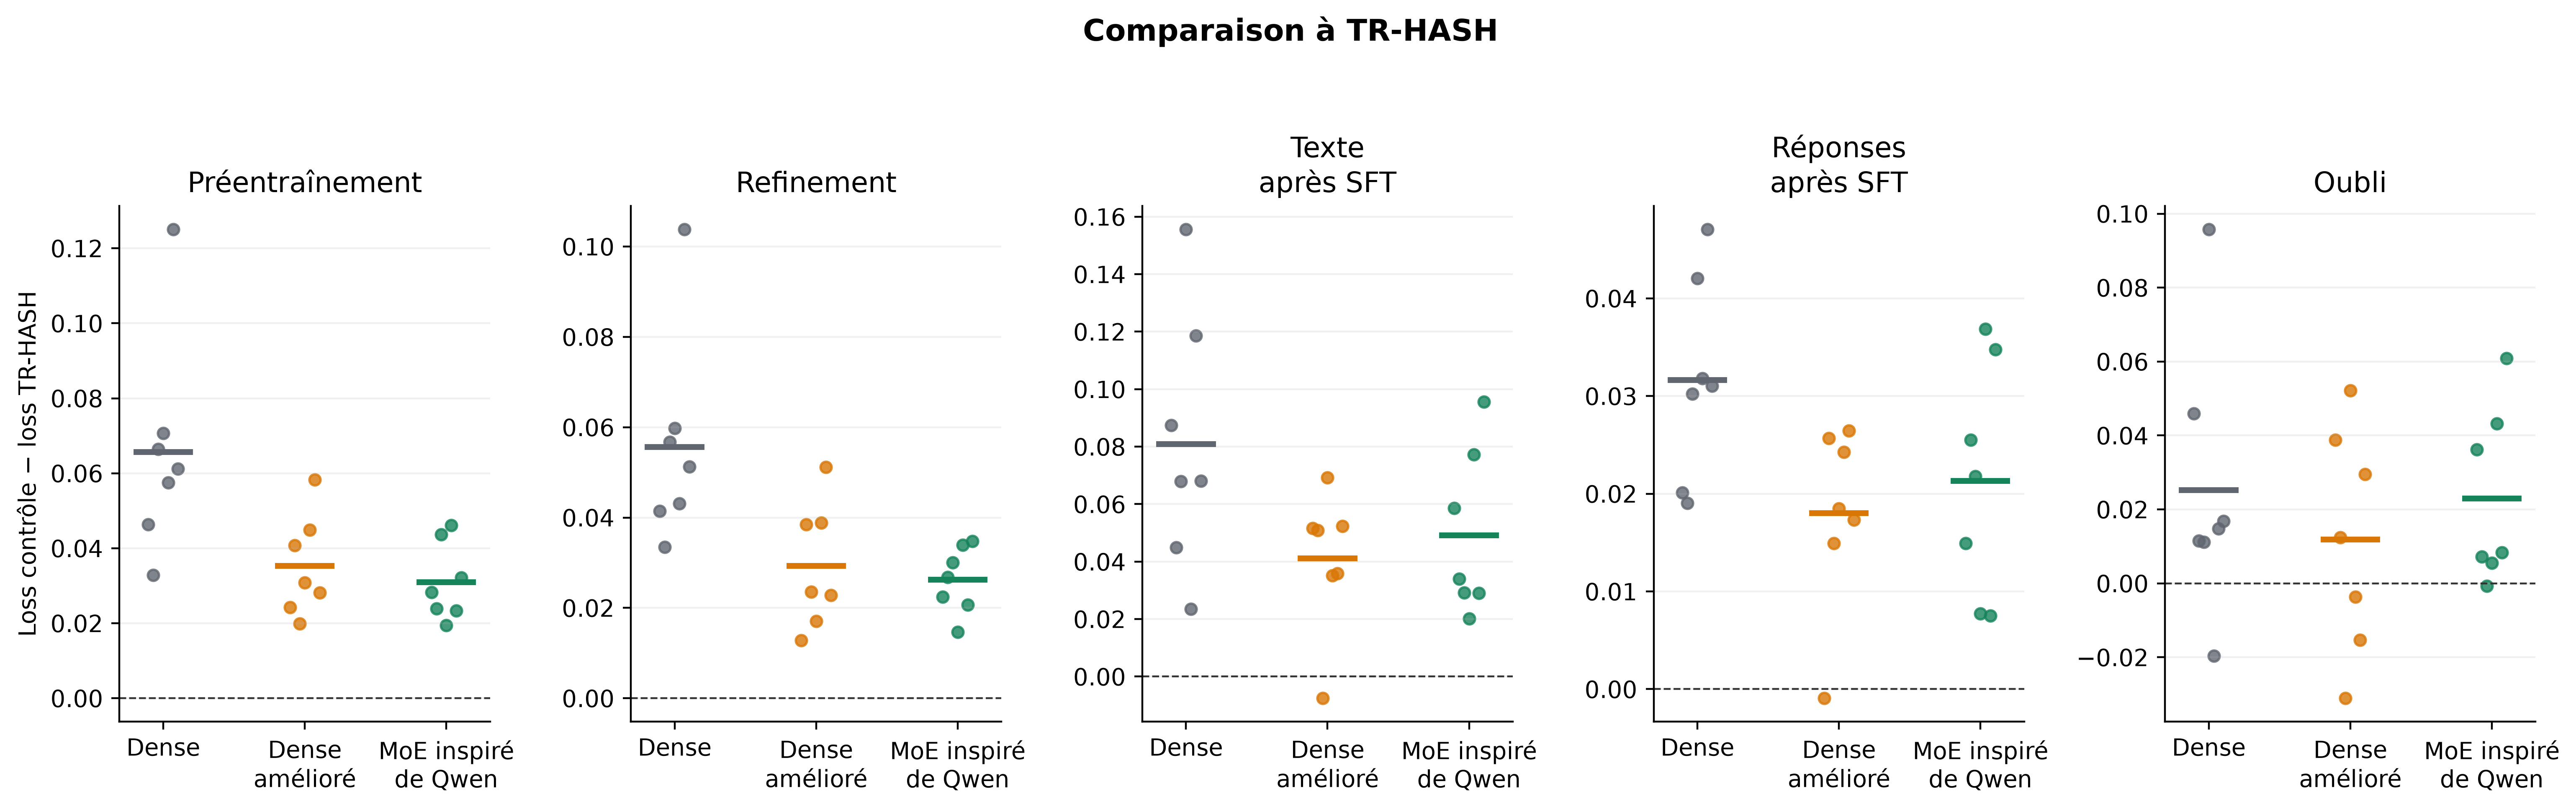
\includegraphics[width=\textwidth]{figures/paired_deltas.png}
\caption{Fresh qualification, paired differences for every seed and metric. The vertical axis is control CE minus \TR{} CE (or the corresponding forgetting difference); positive favors \TR. Dots are the seven development seeds and horizontal marks are their means. The dashed line denotes equality, not the $0.001$-nat success margin. $E$, $D63$, and MoE denote the three fresh controls. No confidence interval is shown.}
\label{fig:paired}
\end{figure}

\begin{figure}[t]
\centering
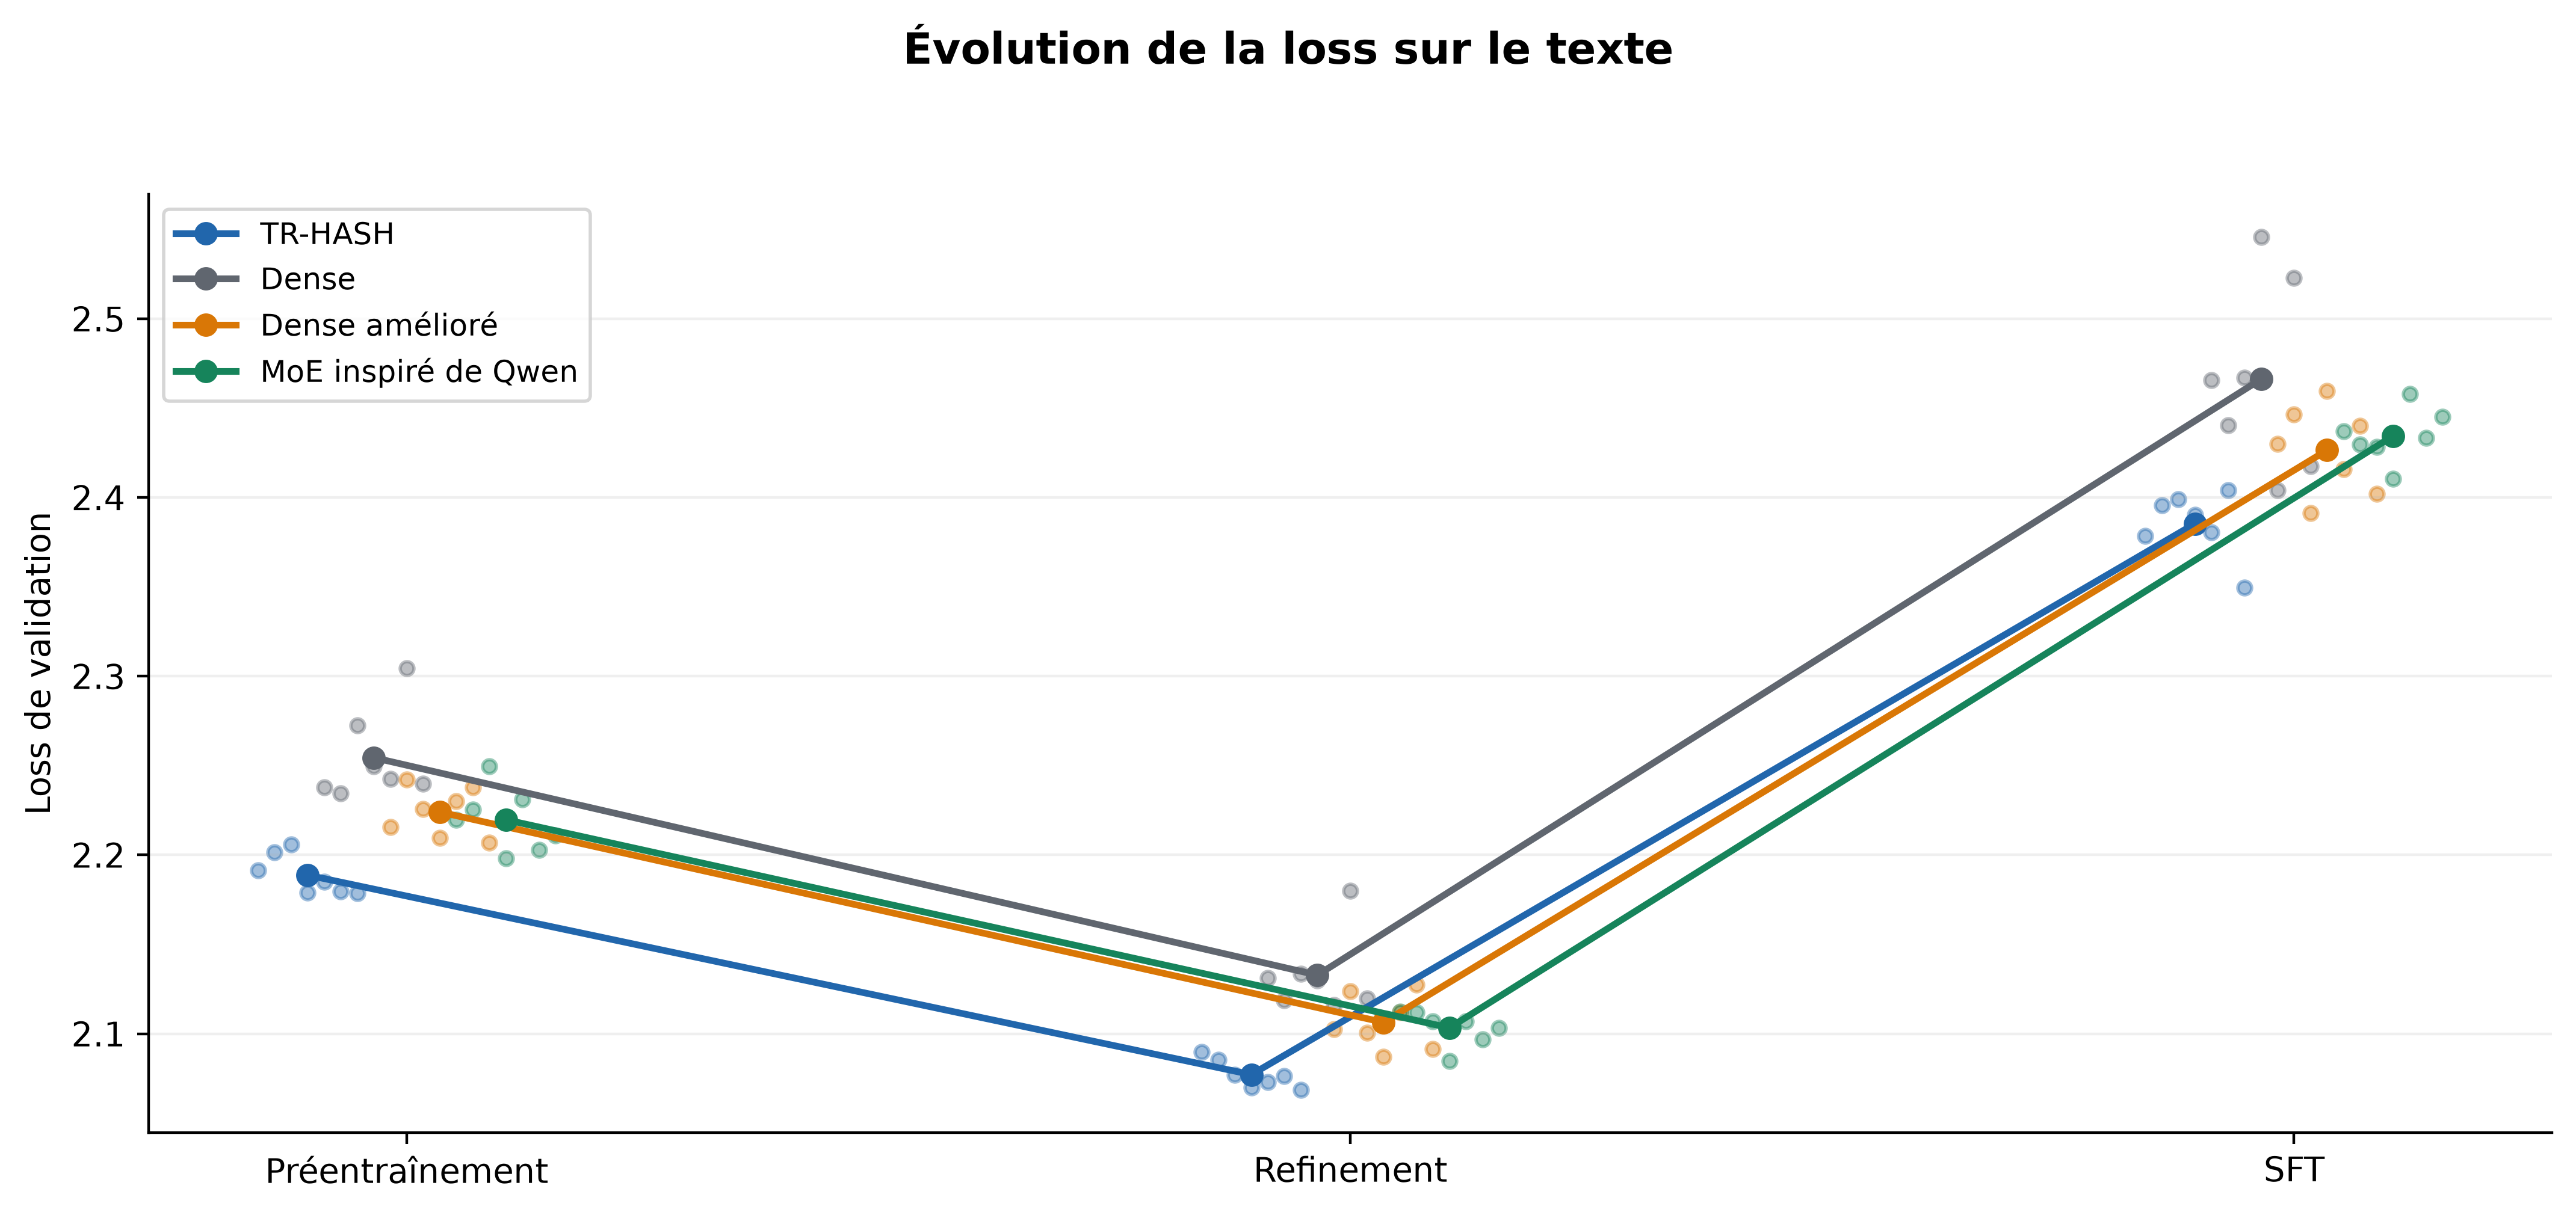
\includegraphics[width=.87\textwidth]{figures/lm_checkpoints.png}
\caption{Held-out language-modeling CE after pretraining, refinement, and SFT. Pale points are seed outcomes; solid points and connecting lines show the seven-seed means at these three measured endpoints. The increase after SFT is the distributional forgetting probe defined in Equation~\ref{eq:forgetting}, not an interpolation of unmeasured validation epochs.}
\label{fig:checkpoints}
\end{figure}

\section{Limitations and interpretation}
\label{sec:limits}
\paragraph{Repeated selection.}
The recipe follows a long exploratory sequence of variants evaluated on the same development seeds and data. Selecting the largest aggregate win count can capitalize on noise and on idiosyncrasies of these examples. Within-round source freezing and a fixed margin do not undo earlier adaptive selection. The reported counts and means are descriptive observations conditional on that process. We do not attach a significance claim, confidence level, probability of superiority, or unseen-seed guarantee to them.

\paragraph{Correlated outcomes and incomplete success.}
The losses are correlated, comparators are shared, and forgetting is a difference of two other measurements. Neither the archive's $97/105$ count nor the fresh grid's $98/105$ count is an independent-trial success rate. Its denominator also depends on a chosen set of metrics and controls. The declared all-comparisons objective is visibly unmet, with reserved confirmation still closed. A convincing general result would require a separately specified confirmation procedure and broader data/model scales, not retrospective relabeling of these development comparisons.

\paragraph{Attribution.}
The original dense baselines differ in attention-head selection and value-input binding as well as FFN organization. The matched $D_{63}$ control removes much of that architectural confounding, but does not identify the separate contributions of two-lag routing, fixed expert weights, the layer $1$ head law, or the first value transformation. The learned router also changes both selection and selected-expert weights and adds an auxiliary loss. Subsequent ablations should vary these mechanisms one at a time with the same data, capacities, initialization controls and full-seed completion rule.

\paragraph{Scale, data and retention meaning.}
This is a tiny byte-level system on narrow text distributions and short instructions. The response objective measures held-out target likelihood rather than instruction-following utility or factual correctness. Shakespeare-to-Alpaca adaptation differs substantially from realistic pretraining and post-training pipelines. The forgetting difference is a specific distributional probe; it is not a general measure of catastrophic forgetting, and no rehearsal advantage, protected expert, or causal account of retained knowledge has been established.

\paragraph{Compute and implementation.}
The reference computes expert outputs and attention heads before masking. No speed, energy or realized-FLOP saving has been measured. Routing sparsity must not be used to advertise an implementation-level efficiency benefit here. Cached inference, optimized dispatch and the framework's domain extensions are separate implementation questions. The scored object is precisely the two-layer, four-query/one-KV, width-$64$ Source63 recipe; larger/deeper variants and extensions to other head counts do not inherit its score.

\paragraph{Other modalities.}
Image, video, detection, speech, and sensor-fusion modules can consume the common routing/attention profile with task-specific positional identities and connectors. Their input topology, masks, capacities and training distributions differ from this text experiment. No validated vision, audio or multimodal accuracy result is supplied by this study, and passing a shape, gradient or serialization test is not such a result.

\paragraph{Provenance boundary.}
The local evidence capsule retains the executed source, selected checkpoints, original metadata, previous-reference evidence and the small historical reference. The executable Source63 JSON and selected checkpoint hashes are verified without changing their bytes. Fourteen documentary temporary Source42 pins were already missing before capsule consolidation; their declarations are retained and the capsule explicitly does not claim complete documentary provenance closure. This limitation should remain visible even when the primary saved metrics and selected checkpoints are internally consistent.

\section{Conclusion}
The deterministic-routing candidate has the lowest five mean losses in both the saved archive and a completed four-model development qualification. It nevertheless misses its all-comparisons objective: the historical $E/C/D$ grid gives $97/105$, while the fresh $E/D/\mathrm{MoE}$ grid gives $98/105$, including five clear losses and two near-equal cases. The learned control uses $0.461\%$ more parameters and matches the candidate's attention transformations, but changes routing weights and the training objective together. These results support further controlled investigation of this exact small recipe; repeated use of the development seeds and data prevents an independent confirmation claim or an extrapolation to other scales and modalities.

\section*{Reproducibility and availability}
The local project includes \texttt{qualification/reference.py} and \texttt{qualification/runner.py}, the frozen source JSON, the saved-reference metadata, and per-file SHA-256 mappings. These local artifacts make the present draft auditable; no public code release, publication, or external review is claimed. The raw data remain identified by pinned upstream URLs and digests, with upstream terms governing their use. Before an external submission, a public artifact package, final authorship information, and any applicable disclosure statements must be completed.

\bibliography{references}
\bibliographystyle{tmlr}

\appendix
\section{Parameter accounting and exact scope}
The embedding contributes $256\cdot64=16{,}384$ parameters and also serves as the output projection. Each attention block contains $64^2$ query parameters, two $64\cdot16$ key/value projections, and a $64^2$ output projection, totaling $10{,}240$. Two per-head RMSNorm scales contribute $32$, and the two hidden pre-normalizers contribute $128$. The FFN contributes $3\cdot64\cdot(128+4\cdot16)=36{,}864$, or the identical count for a dense width-$192$ FFN. Therefore
\begin{equation}
 16{,}384+2(10{,}240+32+128+36{,}864)+64=110{,}976.
\end{equation}
The final $64$ parameters are the output RMSNorm scale. Deterministic route tables and masks are buffers or computed indices, not additional learned parameters. The learned control adds $2(64\cdot4)=512$ router weights. The source uses the same set of trainable parameters throughout all stages; routing does not freeze experts.

Mathematically, an assigned FFN uses shared width $128$ plus two width-$16$ experts, while a dense control uses width $192$. This distinction can matter for an optimized implementation's active work, but it does not override the actual all-expert reference execution. Stored-parameter matching and update-count matching do not imply equal wall-clock work. The manuscript consequently avoids an efficiency or compute-normalized quality claim.

\section{Evidence identities and machine-readable checks}
The historical observations are in \path{artifacts/tr_hash/references/current_best.json}; byte-exact original metadata, scored CSV and executed source strings remain in its reference capsule. The completed four-model records are under \path{artifacts/tr_hash/qualification/run_20261026T204413_039027Z/}. Their \path{results.json} SHA-256 is
\begin{quote}
\small\texttt{9b2f84c58f15e3e900a45d5db7f1cac7}\\
\texttt{798b493f5857400aad755b70c029ceb8}.
\end{quote}
The paper includes the endpoint table \path{results.csv}. The standalone companion notebooks \path{TR_Hash_Qualification.ipynb} and \path{TR_Hash_Research.ipynb} are provided at the repository root for the qualification and further research workflows. The official style's pinned source identity and license provenance are recorded in \path{TMLR_STYLE_PROVENANCE.json}. The capsule has $84$ current-reference checkpoint links and $84$ previous-reference links (overlapping controls), plus $18$ historical checkpoints; these are not counts of independent experiments.

The completed historical Source63 lot contains $14$ fresh trajectories: $10{,}752$ updates and $17{,}342{,}136$ target presentations. An interrupted attempt and a pre-training failure remain separately recorded. Global historical accounting is only a lower bound of $15{,}616$ updates and $25{,}298{,}768$ target presentations; the interrupted attempt prevents an exact total-cost claim. Partial trajectories are excluded from result tables.

\section{Required follow-up comparisons}
A useful next matrix would keep the same recipe, data order, masks and optimizer schedule while separately testing (i) original versus Source63 head selection with the same FFN; (ii) identity versus layer $0$ value permutation with matched heads; (iii) one-lag versus two-lag expert identities; and (iv) learned routing with and without the declared balancing coefficient. These are proposed interventions, not reported outcomes. The learned router's extra $512$ parameters should be disclosed in every comparison, and a further capacity-adjusted control could test whether that small difference matters.

After development choices are frozen, confirmation should use separately specified untouched examples and report all completed models and seeds. The seven familiar development seeds cannot alone establish unseen-initialization robustness. Any domain extension should define its positional-ID ordering, sequence boundaries, masks and retained task-specific components before training, then obtain its own measurements. No numerical conclusion in this manuscript substitutes for those steps.


\section{Additional recorded qualification figures}
\label{sec:figures}
All panels below come from the completed $28$-trajectory development run. Pale lines or points represent seeds and heavier marks represent means. These are descriptive plots of reused development data, not independent confirmation or confidence intervals.

\begin{figure}[!htbp]
\centering
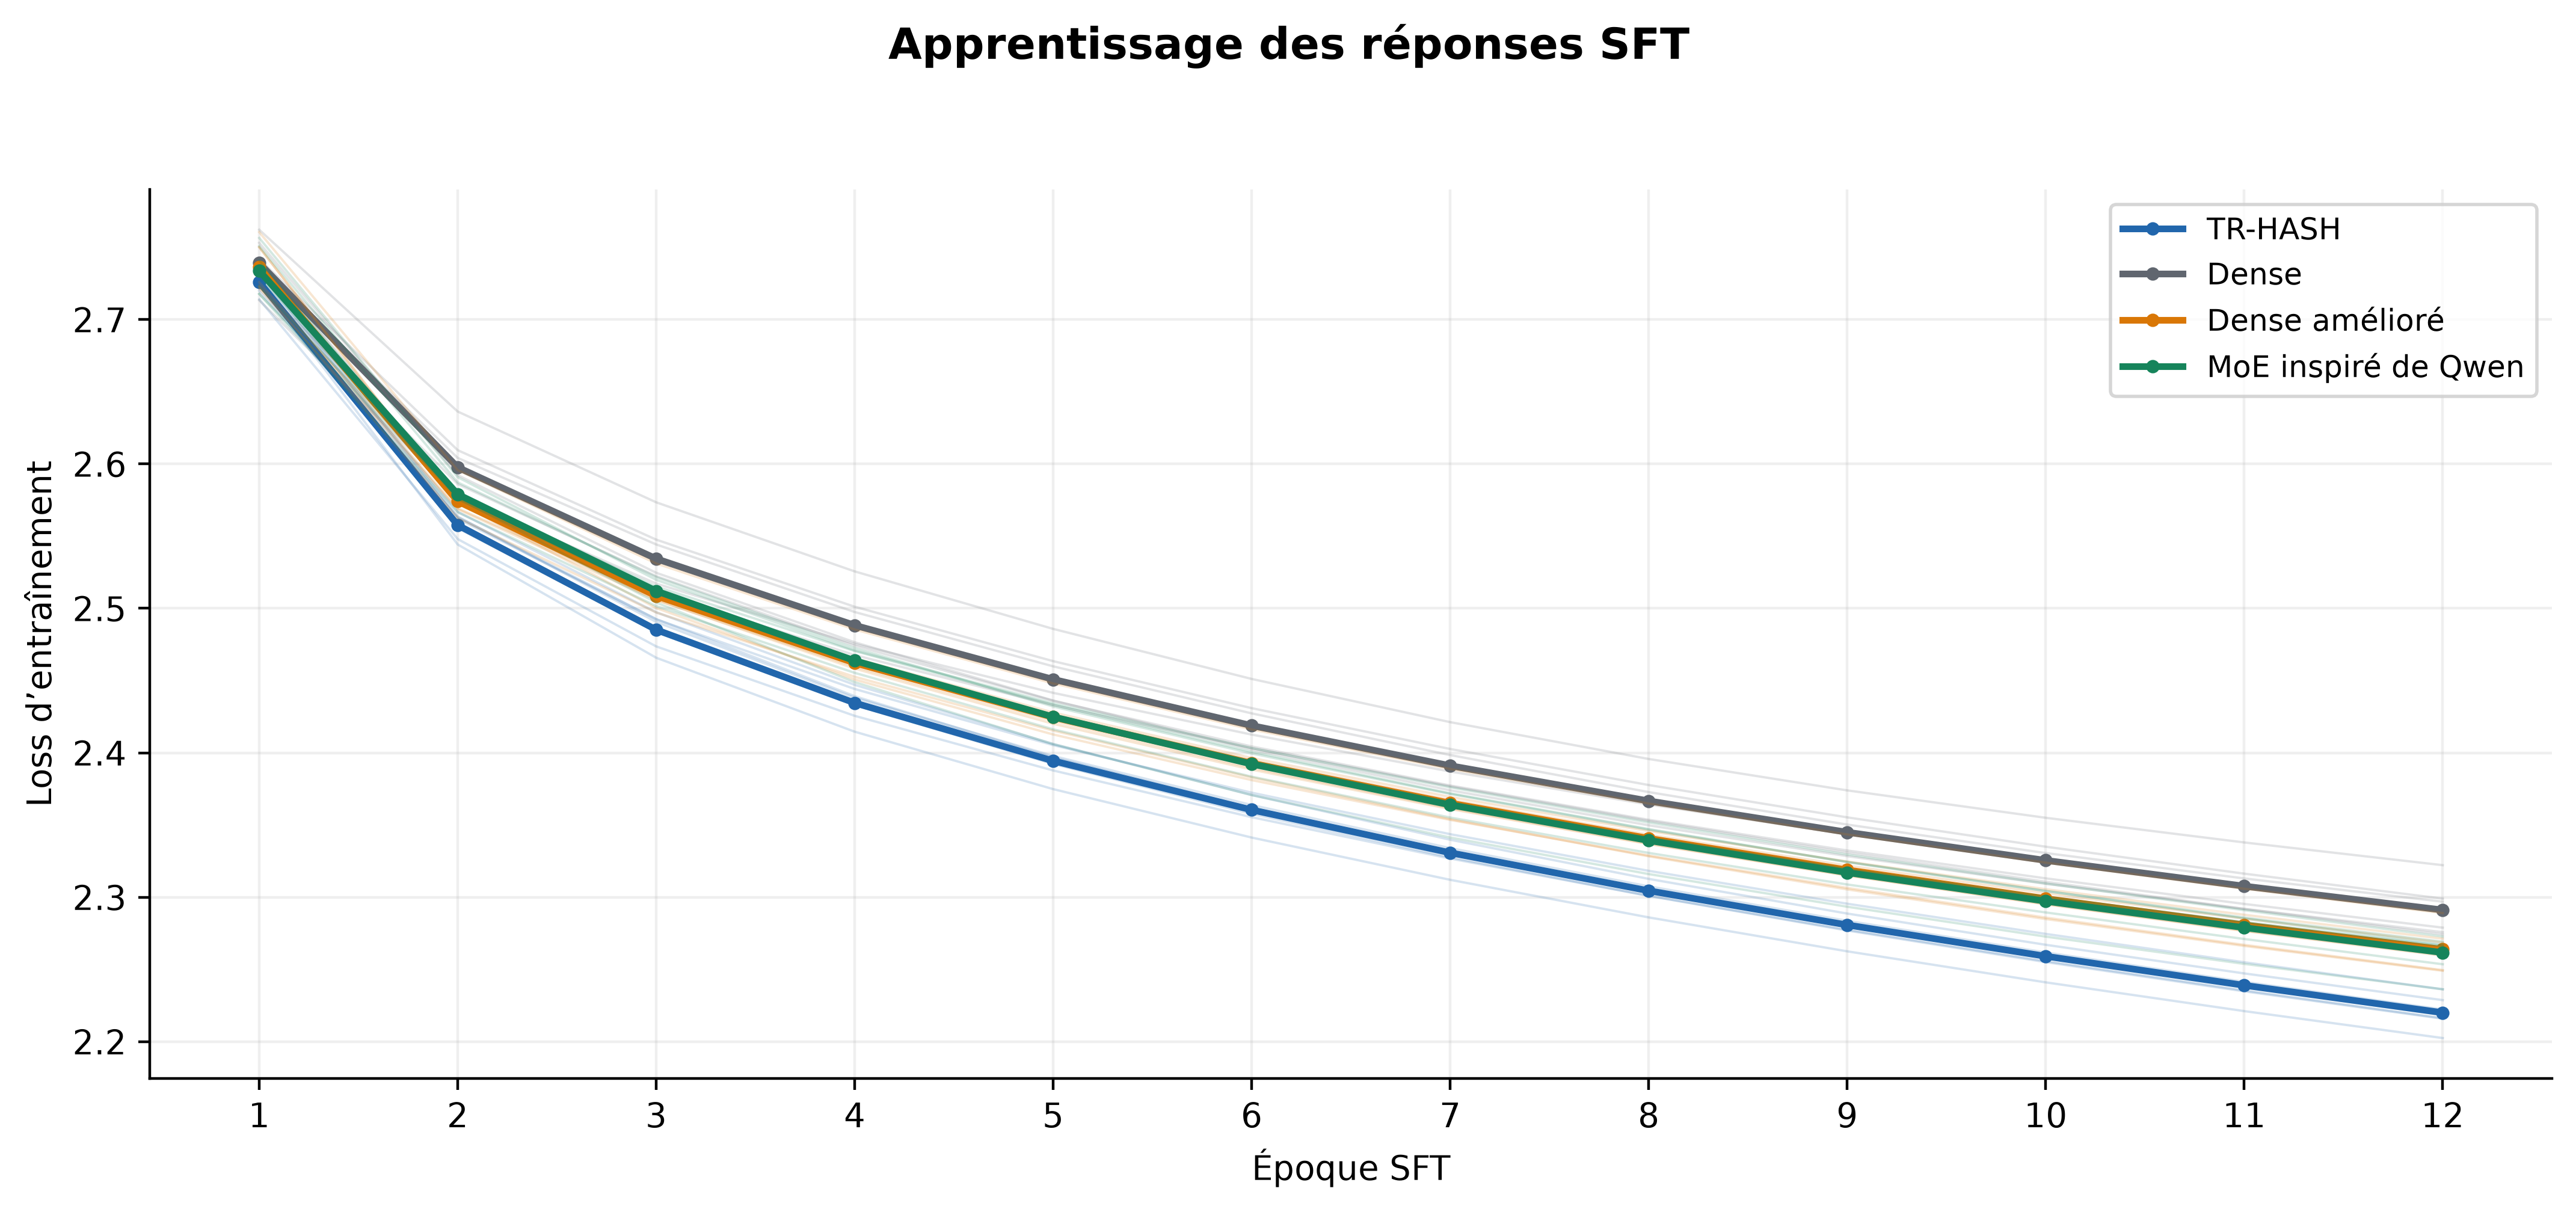
\includegraphics[width=.85\textwidth]{figures/sft_training_ce.png}
\caption{Twelve recorded SFT epoch training cross-entropies, excluding the balancing auxiliary term. Thin curves are individual seeds and thick curves are seven-seed means. These are training measurements; no intermediate validation curve is inferred.}
\label{fig:sft}
\medskip
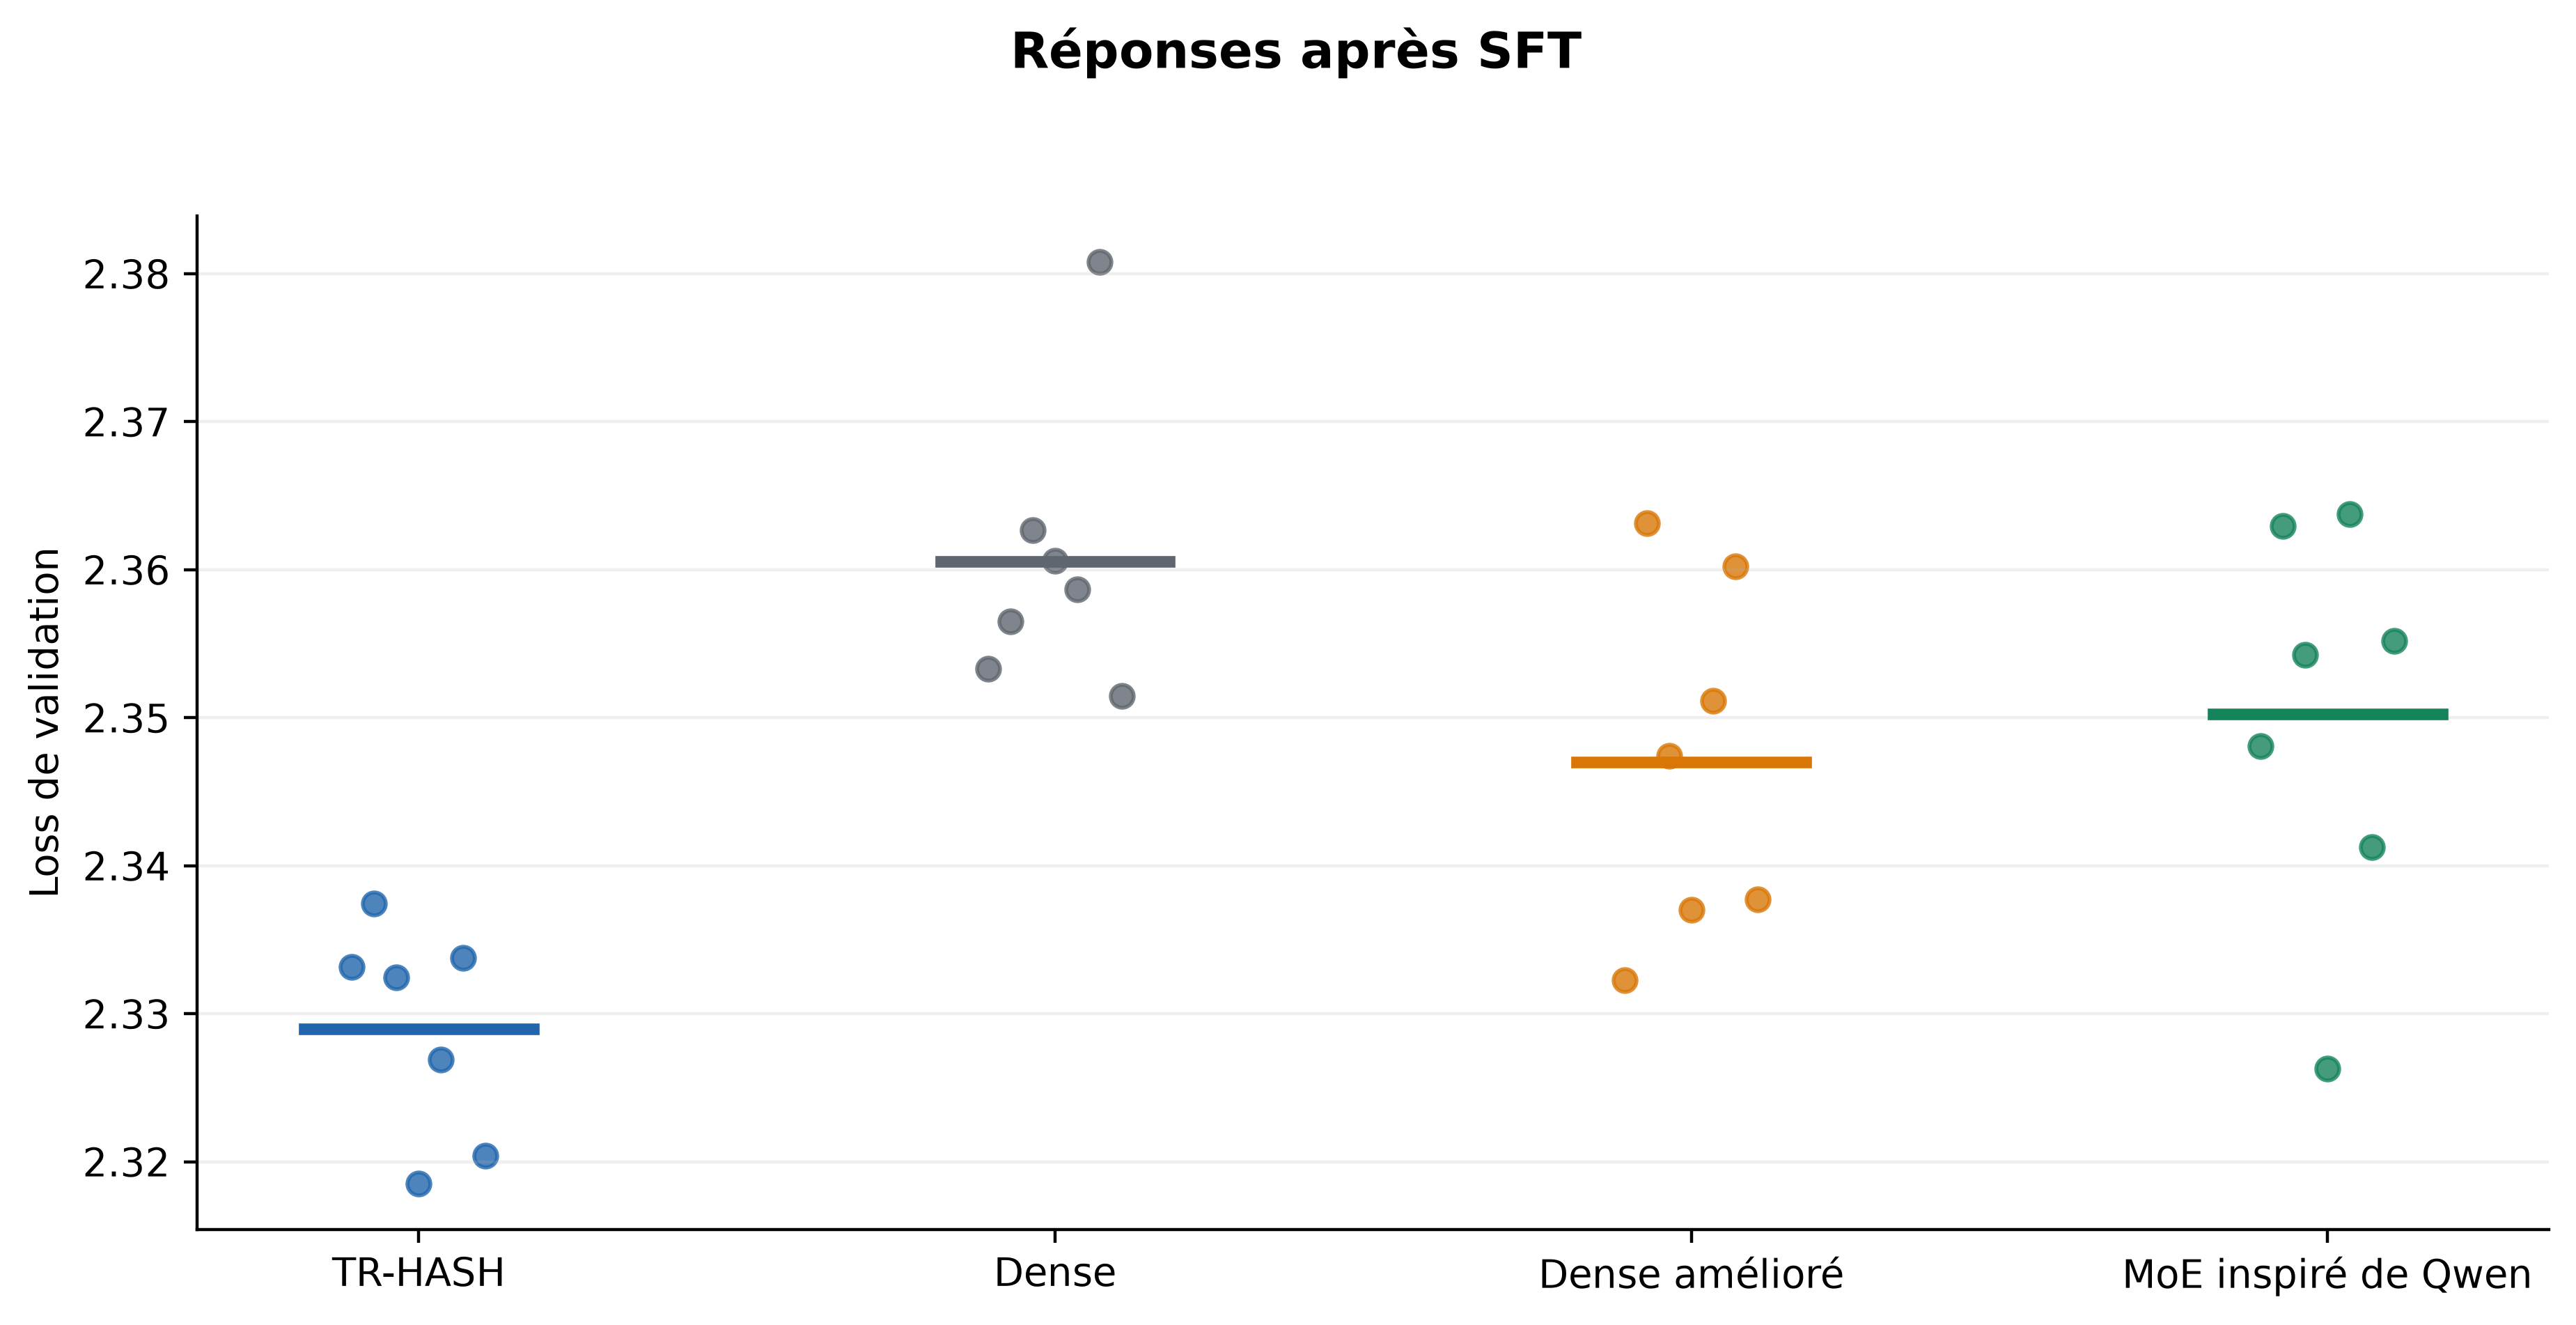
\includegraphics[width=.85\textwidth]{figures/final_responses.png}
\caption{Final response-validation CE, with one point per development seed and a horizontal mean for each model. Lower values indicate higher likelihood of the held-out target answers, not an assessed preference or generation-quality score.}
\label{fig:responses}
\end{figure}

\begin{figure}[!htbp]
\centering
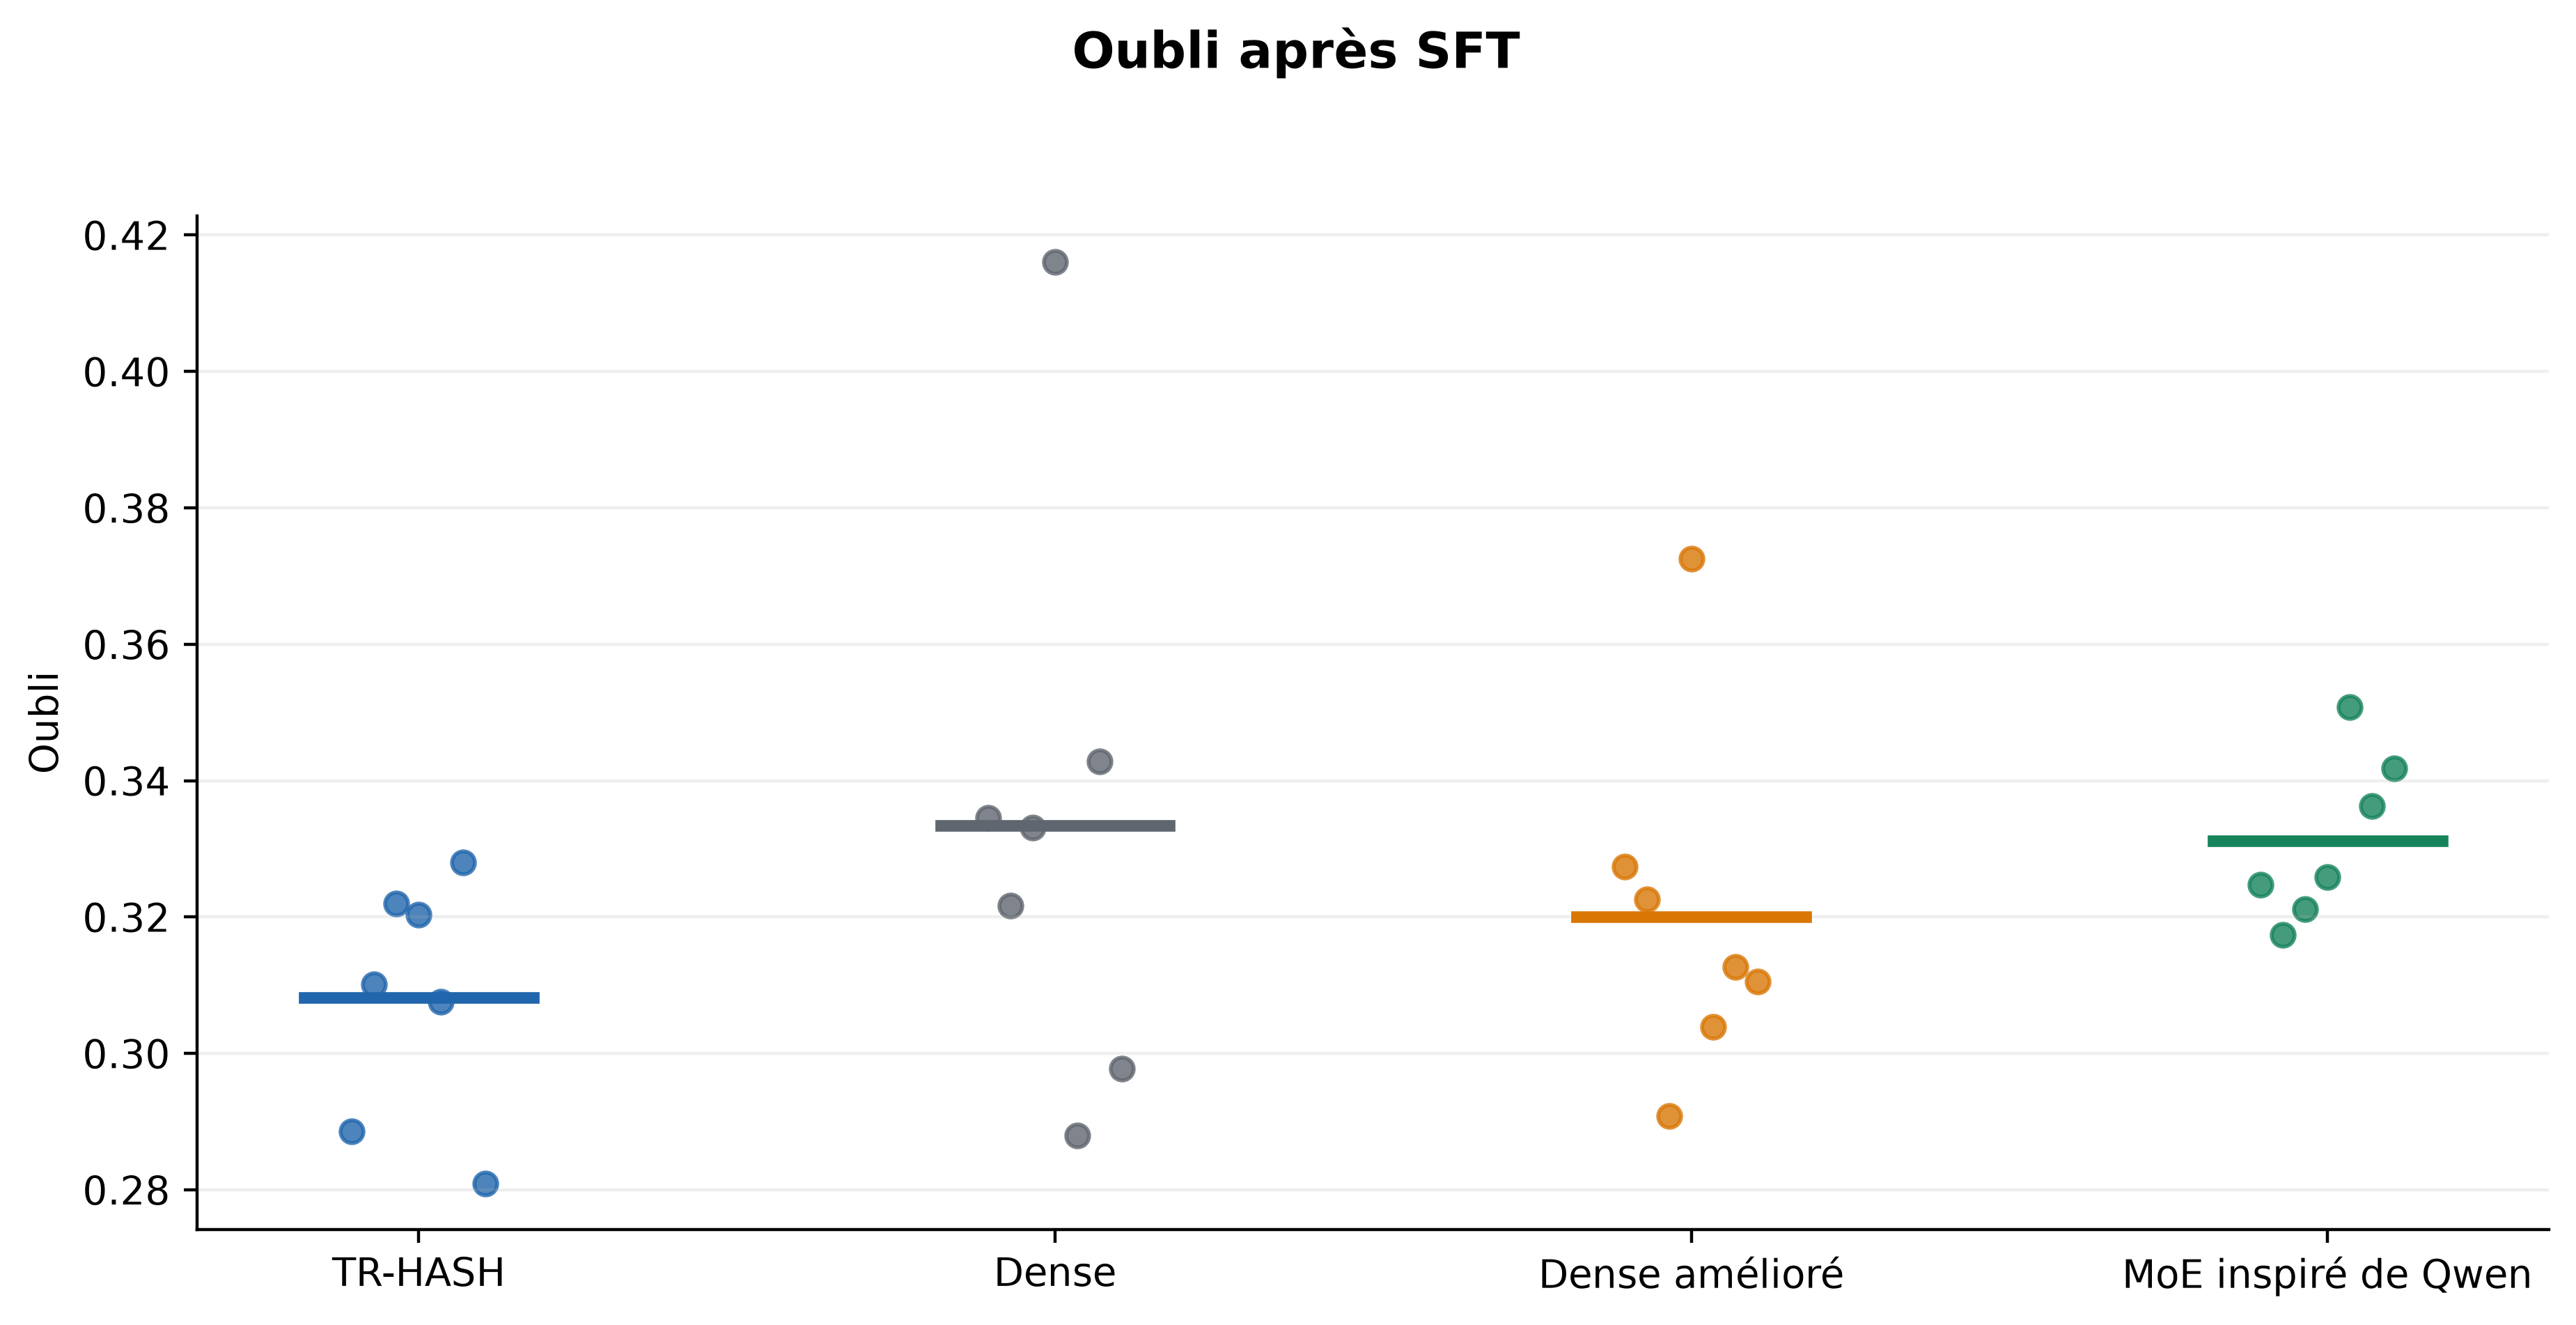
\includegraphics[width=.82\textwidth]{figures/forgetting.png}
\caption{Forgetting (``Oubli'' in the plot): final LM CE minus post-refinement LM CE. Points show the seven development seeds and bars their means. Lower is preferred, interpreted alongside the absolute LM endpoints.}
\label{fig:forgetting}
\medskip
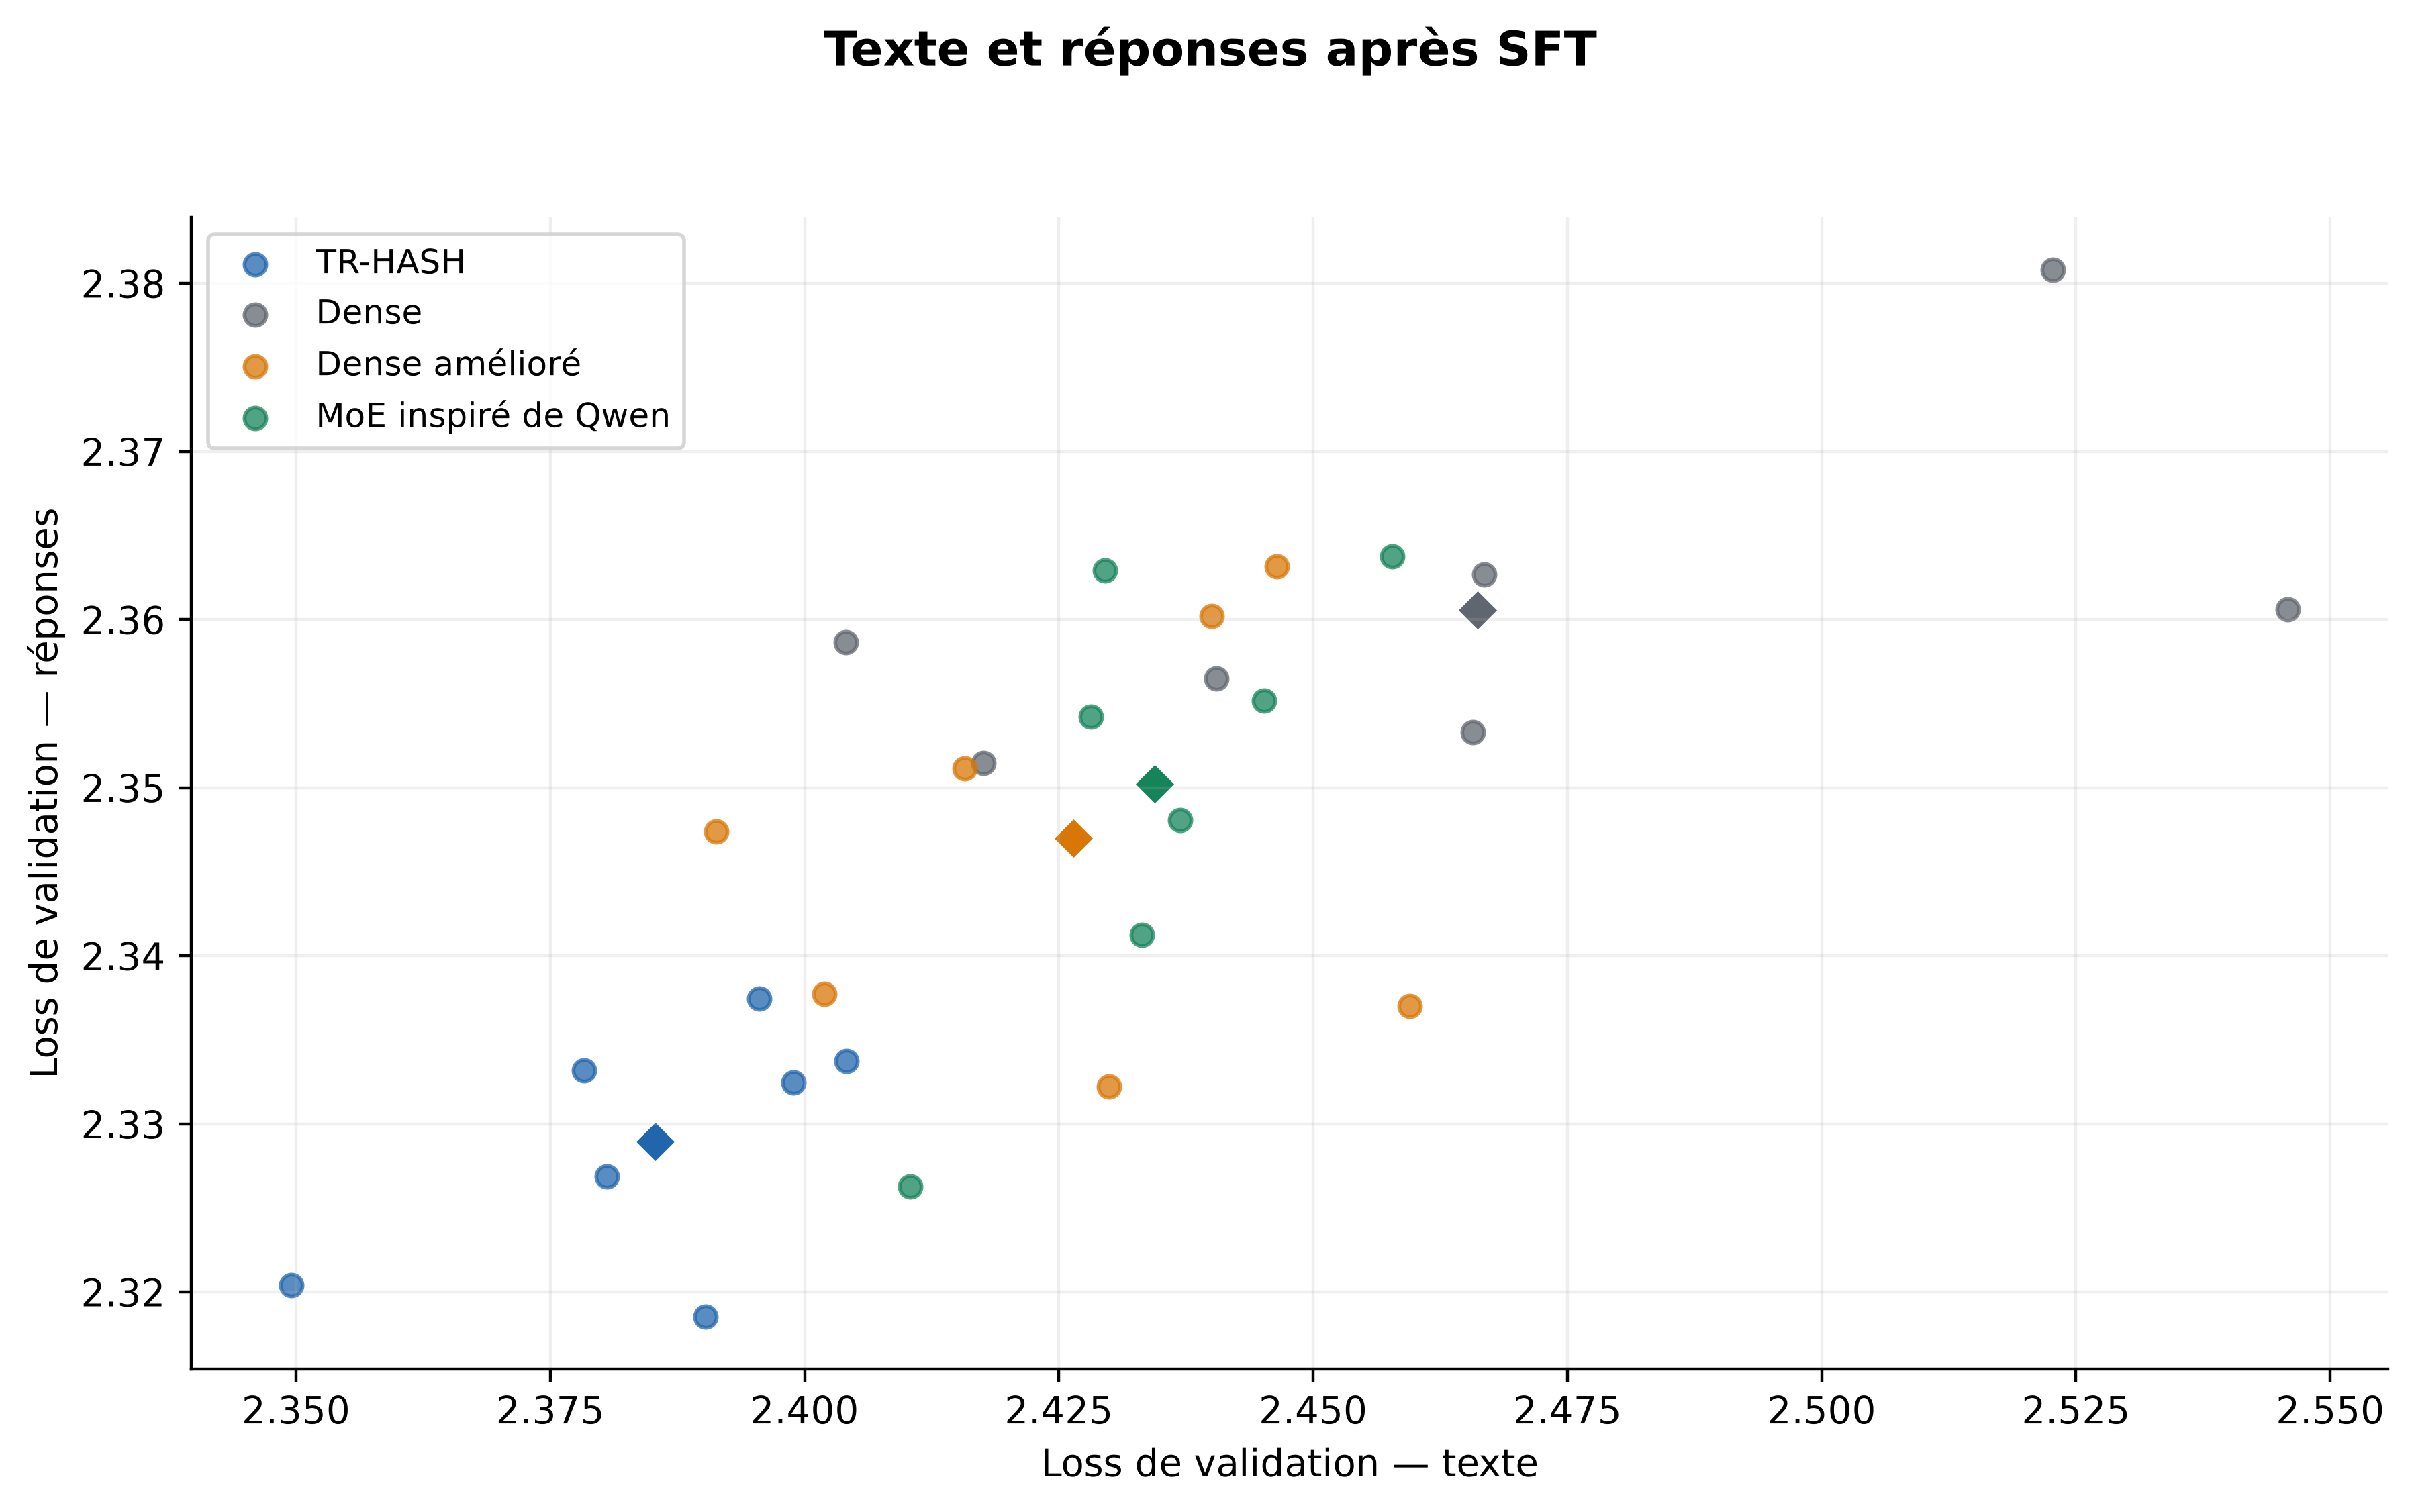
\includegraphics[width=.77\textwidth]{figures/final_text_vs_responses.png}
\caption{Final LM CE (horizontal axis) against final response CE (vertical axis). Seven points per model show the development seeds; diamonds mark model means. Lower left is favorable on these two measured objectives. The plot does not establish a Pareto guarantee across seeds or unmeasured tasks.}
\label{fig:tradeoff}
\end{figure}

\end{document}
